\documentclass[12pt]{article}

\usepackage[utf8]{inputenc}
\usepackage{geometry}
\geometry{a4paper,scale=0.75}
\linespread{1.5}
\usepackage{graphicx} 
\usepackage{float} 
\usepackage{subfig} 
\usepackage{enumerate}
\usepackage{enumitem}
\usepackage{amsmath}
\usepackage{array}
\usepackage{booktabs}
\usepackage{multirow}
\usepackage{amsfonts}
\usepackage[english]{babel}
\usepackage{amsthm}
\usepackage{dcolumn}
\usepackage{multicol}
\usepackage{stfloats}
\usepackage{lscape}
\usepackage[figuresright]{rotating}
\RequirePackage{pdflscape}
\usepackage[toc,page]{appendix}
\usepackage{geometry}
\usepackage{longtable}
\usepackage{comment}
\usepackage{xcolor}

% -------- enumerated sub-labels (a), (b), … --
\usepackage{enumitem}
\setlist[enumerate,1]{label=(\alph*),ref=\alph*}
% ---------------------------------------------

\usepackage{hyperref}
\hypersetup{hidelinks,
	colorlinks=true,
	allcolors=black,
	pdfstartview=Fit,
	breaklinks=true}
\usepackage{csquotes}
\usepackage{natbib}
\bibliographystyle{apalike}
\newtheorem{definition}{Definition}
\newtheorem{theorem}{Theorem}
\newtheorem{proposition}[theorem]{Proposition}
\newtheorem{lemma}[theorem]{Lemma}
\newtheorem{corollary}[theorem]{Corollary}
\newtheorem*{remark}{Remark}
\newtheorem{example}{Example}
\newtheorem{exercise}{Exercise}
\newtheorem{assumption}{Assumption}[section] % number within sections


\begin{document}

\begin{center}
    ECON 3123: Macroeconomic Theory I\\
    {\large \textbf{Tutorial Note 3: Investment and Financial Market}}\\
    Teaching Assistant: Harlly Zhou
\end{center}

\subsection*{Money Supply and Demand}
\paragraph{Definition of Money}
$M1$: Currency and checkable deposits (Liquid assets)

$M2$: Less liquid assets

A financial asset is \textbf{liquid} if it can be quickly used to buy goods and services.

\begin{remark}
	As emphasized by Perry Mehrling (Columbia University) in his Money and Banking course, money is best analyzed as a \emph{hierarchy} rather than by a single definition. Under the gold standard, gold sits at the apex as the ultimate settlement asset. Below gold are national currencies, whose values are defined by their convertibility into gold at a fixed parity. Bank deposits lie further down: they are promises to deliver currency on demand and ordinarily exchange at par. In stress—e.g., during recessions when banks face currency shortages—par convertibility may fail, and deposits can trade at a discount to currency or be temporarily suspended. Lower still are various securities, which are the least money-like in this ordering.
\end{remark}

\begin{exercise}
    \begin{enumerate}[label=(\arabic*)]
		\item Which of the following statements about M1 and M2 is true?
		\begin{enumerate}[label=\Alph*]
			\item Demand deposits are not part of M1.
			\item M2 is more liquid than M1.
			\item M1 is larger than M2.
			\item Savings deposits are part of M2.
		\end{enumerate}
		\item In some countries, prices in stores are listed in terms of U.S. dollars, rather than in units of the local currency. That's most likely because
		\begin{enumerate}[label=\Alph*.]
			\item the country's political system is unstable.
			\item interest rates are higher using U.S. dollars than using the local currency.
			\item there is no other store of value. 
			\item the country has experienced high rates of inflation.
		\end{enumerate}
	\end{enumerate}
\end{exercise}

\paragraph{Who is supplying money?}
\textbf{Central banks} typically change the supply of money, $M^S$, by buying or selling government bonds in the bond market, open to everyone. 

Expansion vs Contraction: Whether more money is circulating in the market. 
\begin{itemize}
	\item Expansionary policy: More money is circulating. Central bank \textbf{buys} bond and \textbf{pays money} to the sellers.
	\item Contractionary policy: Less money is circulating. Central bank \textbf{sells} bond and \textbf{gets money} to the sellers. 
\end{itemize}

\begin{exercise}
	\begin{enumerate}[label=(\arabic*)]
		\item Suppose you read in the paper that the Federal Reserve plans to expand the money supply. The Fed is most likely to do this by
		\begin{enumerate}[label=\Alph*]
			\item printing more currency and distributing it.
			\item purchasing government bonds from the public.
			\item selling government bonds to the public.
			\item buying newly issued government bonds directly from the government itself.
		\end{enumerate}
		\item A developing country does not have enough taxes to cover its expenditures and is unable to borrow. This government would be most likely to cover its deficit by
		\begin{enumerate}[label=\Alph*]
			\item purchasing government bonds from the public.
			\item selling government bonds to the public.
			\item selling newly issued government bonds directly to the central bank.
			\item buying newly issued government bonds directly from the central bank.
		\end{enumerate}
	\end{enumerate}
\end{exercise}

\paragraph{Functions of Money}
Money has three functions:
\begin{itemize}
	\item medium of exchange: an instrument for transaction.
	\item store of value: an asset preserving purchasing power.
	\item unit of account: a numeraire measuring financial items.
\end{itemize}

Money is liquid, and can be directly used for transaction, while other financial assets may not. However, other financial assets provide (potential) positive \textbf{financial income}, including interest rate income. Other financial assets bear larger risk than money, but the return can be higher.

\begin{exercise}
    Compared with money, bonds have
	\begin{enumerate}[label=\Alph*.]
		\item less risk and less liquidity.
		\item less risk and more liquidity.
		\item more risk and less liquidity.
		\item more risk and more liquidity.
	\end{enumerate}
\end{exercise}

\paragraph{Money Demand}
Consider a one-year zero-coupon risk-free bond with face value \$100. Suppose you invest $\$ P_B$ now. The rate of return of this bond is the interest rate:
\begin{align*}
	i = \frac{100 - P_B}{P_B} \iff P_B = \frac{100}{1 + i}.
\end{align*}
$P_B$ is called the bond price.

Suppose the interest rate increases. Then the demand for money decreases (why?). We assume the following money demand function:
\begin{align*}
	M^D = \$ Y L(i)
\end{align*}
where $Y$ denotes the nominal \textbf{income} (we will see why I emphasize this) and $L(i)$ is a \textbf{decreasing} function of interest rate $i$. 

One unit of money travels many times across different people. The nominal GDP should be exactly the amount of money times the number of times it travels. Here is the \textbf{quantity theory of money}:
\begin{align*}
	M^D V = \$ Y
\end{align*}
where $V$ is the \textbf{velocity} of money, characterizing how fast money should travel across people.

\begin{example}
	Chapter 4, Question 5 in Blanchard, Olivier (2021), \textit{Macroeconomics}, 8th ed., Pearson.

	Suppose that a person's wealth is \$50,000 and that her yearly income is \$60,000. Also suppose that her money demand function is given by
	\[M^d = \$ Y (0.35 - i).\]

	\begin{enumerate}[label=(\alph*)]
		\item Derive the demand for bonds. Suppose that the interest rate increases by 10 percentage points. What is the effect on her demand for bonds?
		\vspace{36pt}
		\item What are the effects of an increase in wealth on her demand for money and her demand for bonds? Explain in words.
		\vspace{36pt}
		\item What are the effects of an increase in income on her demand for money and her demand for bonds? Explain in words.
		\vspace{36pt}
		\item Consider the statement ``When people earn more money, they obviously will hold more bonds.'' What is wrong with this statement?
		\vspace{36pt}
	\end{enumerate}
\end{example}

\subsection*{Equilibrium}
The equilibrium in the money market is such that 
\[M^S = M^d,\]
where money supply is determined by the central bank and money demand is the relationship between money, nominal income, and interest rate. 

\begin{figure}[htp]
    \centering
    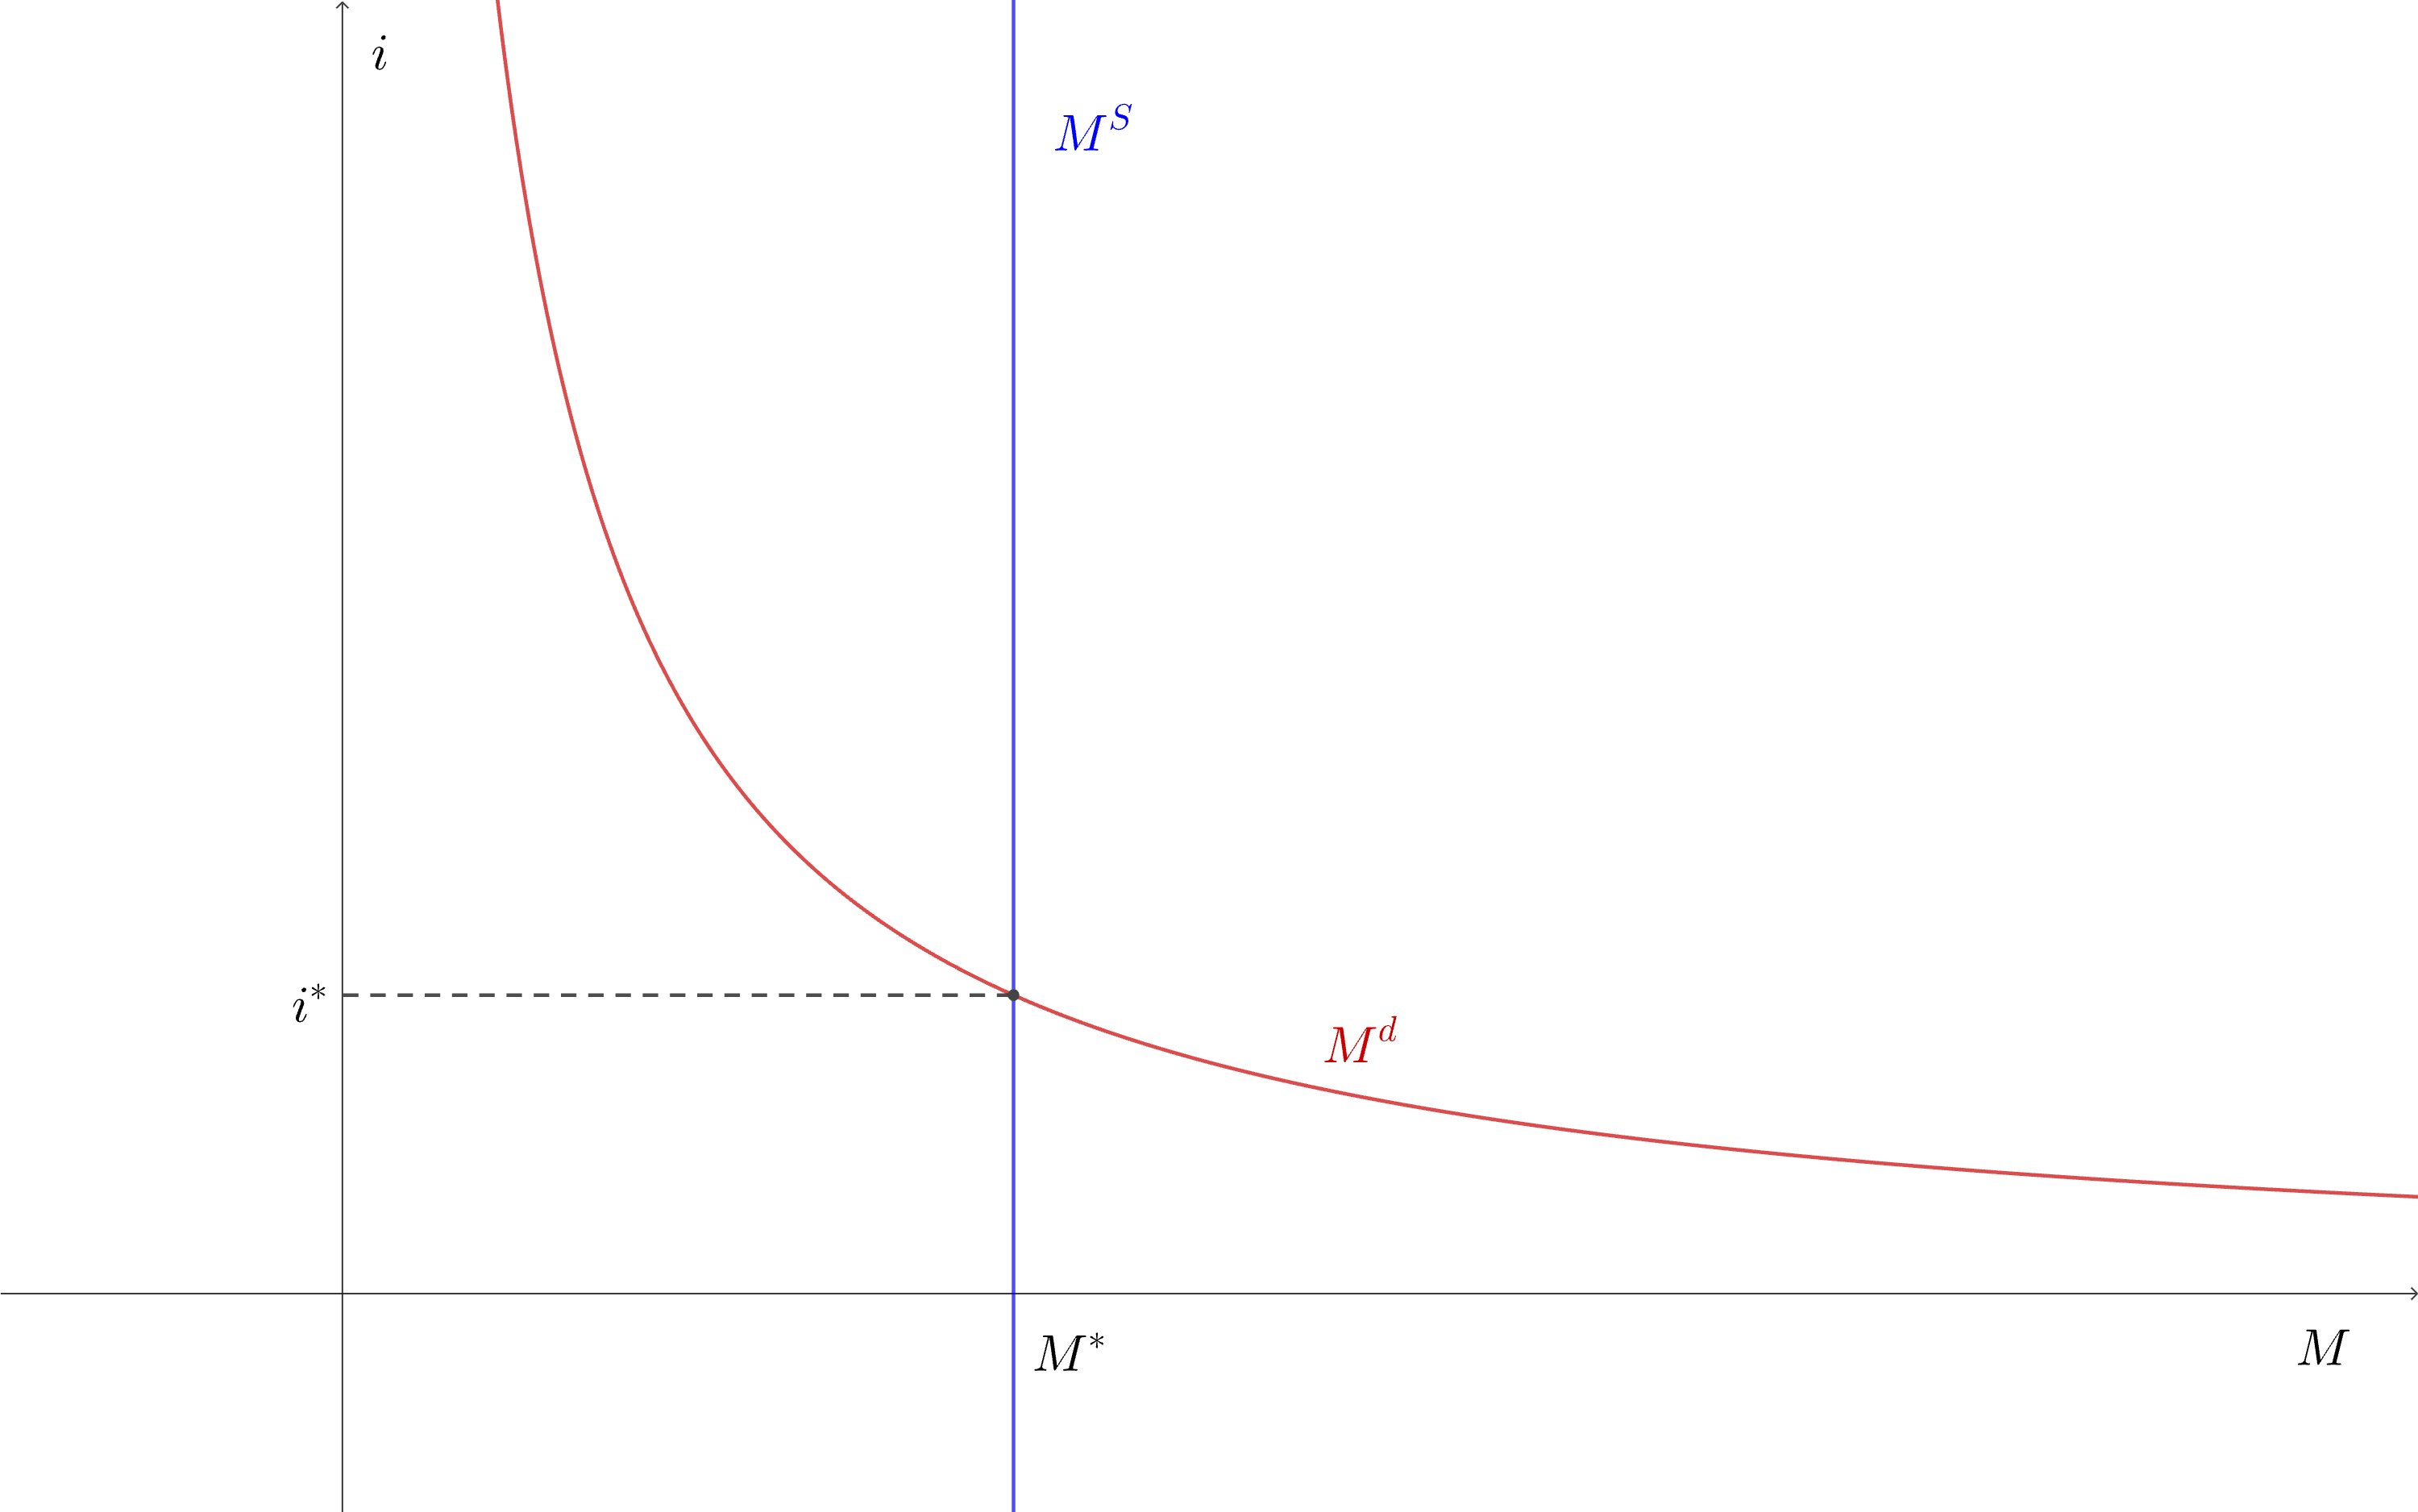
\includegraphics[width=0.5\textwidth]{money_eqm_01.png}
    \caption{Equilibrium in Money Market}
    \label{fig:money_eqm_01}
\end{figure}
Figure \ref{fig:money_eqm_01} shows the equilibrium interest rate in the money market. Since the central bank determines money supply, it is a vertical line. As was discussed, $M^d$ is decreasing in $i$.

\paragraph{Contractionary Monetary Policy}
\begin{itemize}
	\item In the money market, the money supply decreases. Figure \ref{fig:money_eqm_02} shows that, we will have a higher equilibrium interest rate.
	\item In the bond market, the central bank sells bond in the open market. The supply of bond increases, so that the bond price decreases. Recall the bond price formula:
	\[P_B = \frac{\text{Face Value}}{1 + i}.\]
	The interest rate increases.
\end{itemize}
The change of the equilibrium interest rate matches in the two markets.

\begin{figure}[htp]
    \centering
    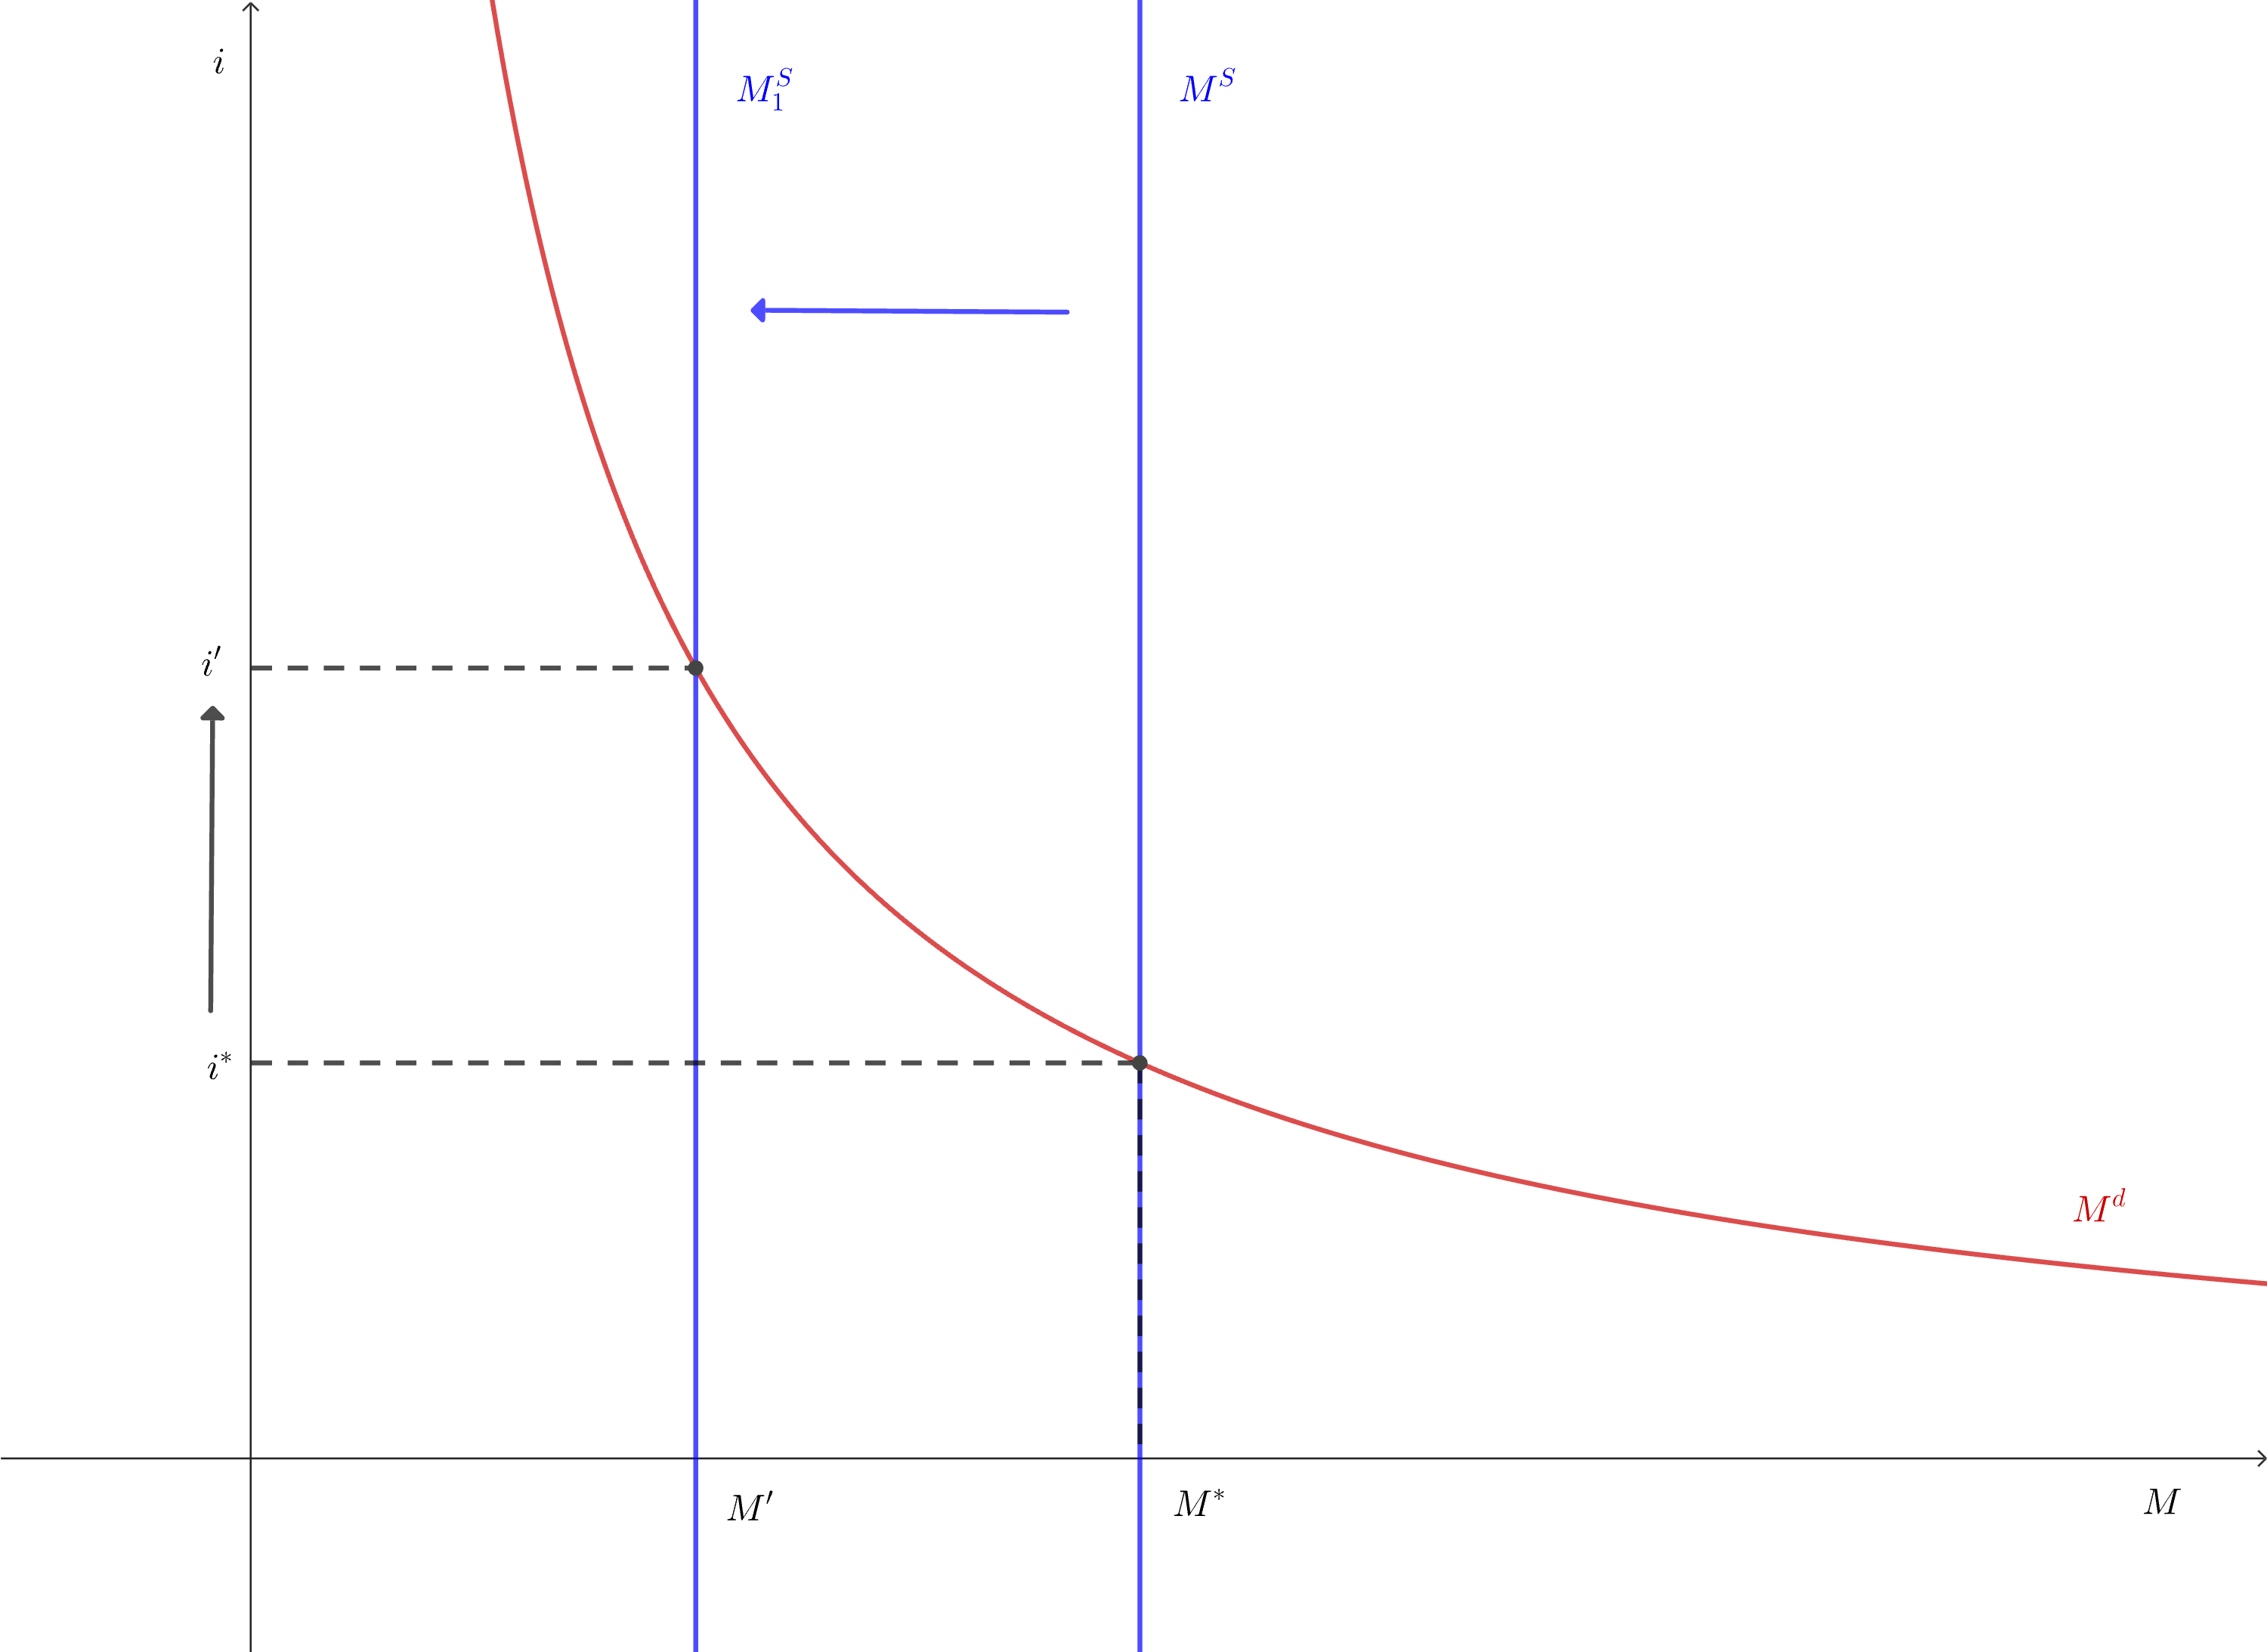
\includegraphics[width=0.5\textwidth]{money_eqm_02.png}
    \caption{Contractionary Monetary Policy}
    \label{fig:money_eqm_02}
\end{figure}

\paragraph{Lower Income}
\begin{itemize}
	\item In the money market, the money demand decreases. Figure \ref{fig:money_eqm_03} shows that, we will have a lower equilibrium interest rate.
	\item In the bond market, the demand for bond increases due to the substitutability between money and bond. Therefore, the bond price increases. The interest rate, as a result, decreases. 
\end{itemize}
The change of the equilibrium interest rate matches in the two markets.

\begin{figure}[htp]
    \centering
    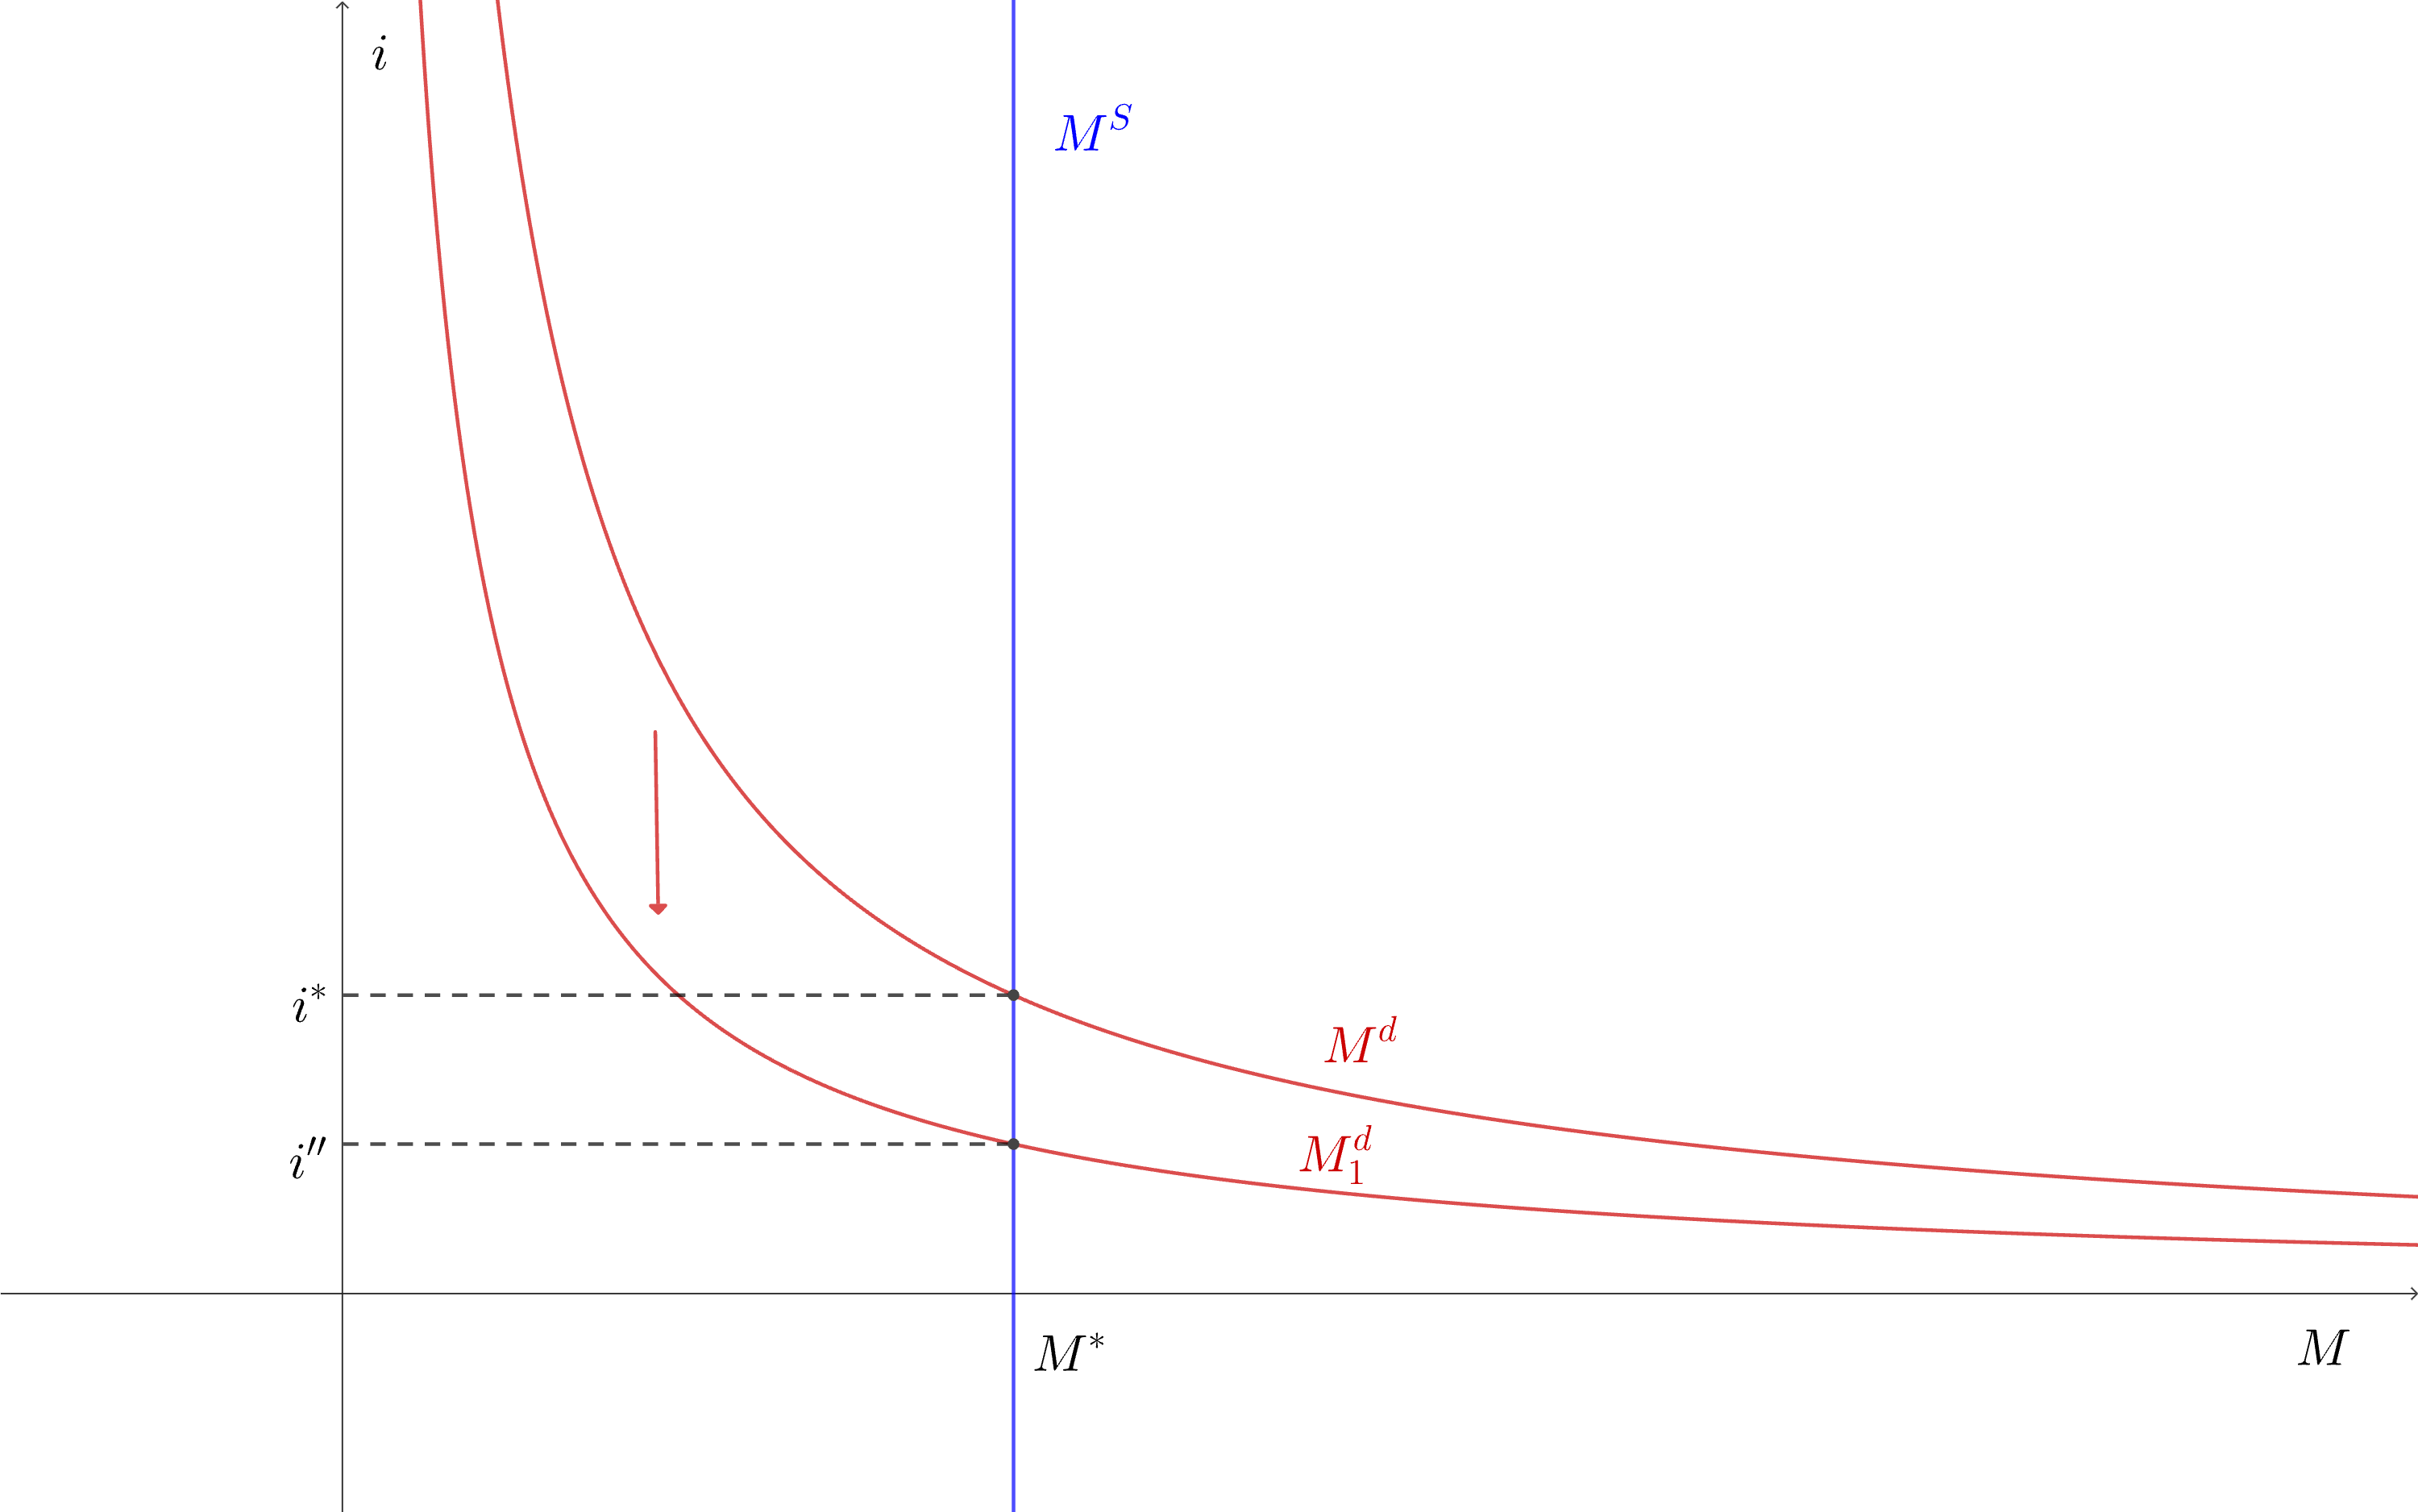
\includegraphics[width=0.5\textwidth]{money_eqm_03.png}
    \caption{Lower Income}
    \label{fig:money_eqm_03}
\end{figure}

\begin{exercise}
	Chapter 4, Question 9 in Blanchard, Olivier (2021), \textit{Macroeconomics}, 8th ed., Pearson.
\end{exercise}

\subsection*{Liquidity Trap}
The central bank can choose the interest rate by changing $M^S$ as long as $i\geq 0$. However, when the \textbf{zero lower bound} (ZLB) is touched, as in \ref{fig:zlb}, increasing $M^S$ cannot lower nominal interest rate any more. Unconventional monetary policy will be used, such as quantitative easing.

\begin{figure}[htp]
    \centering
    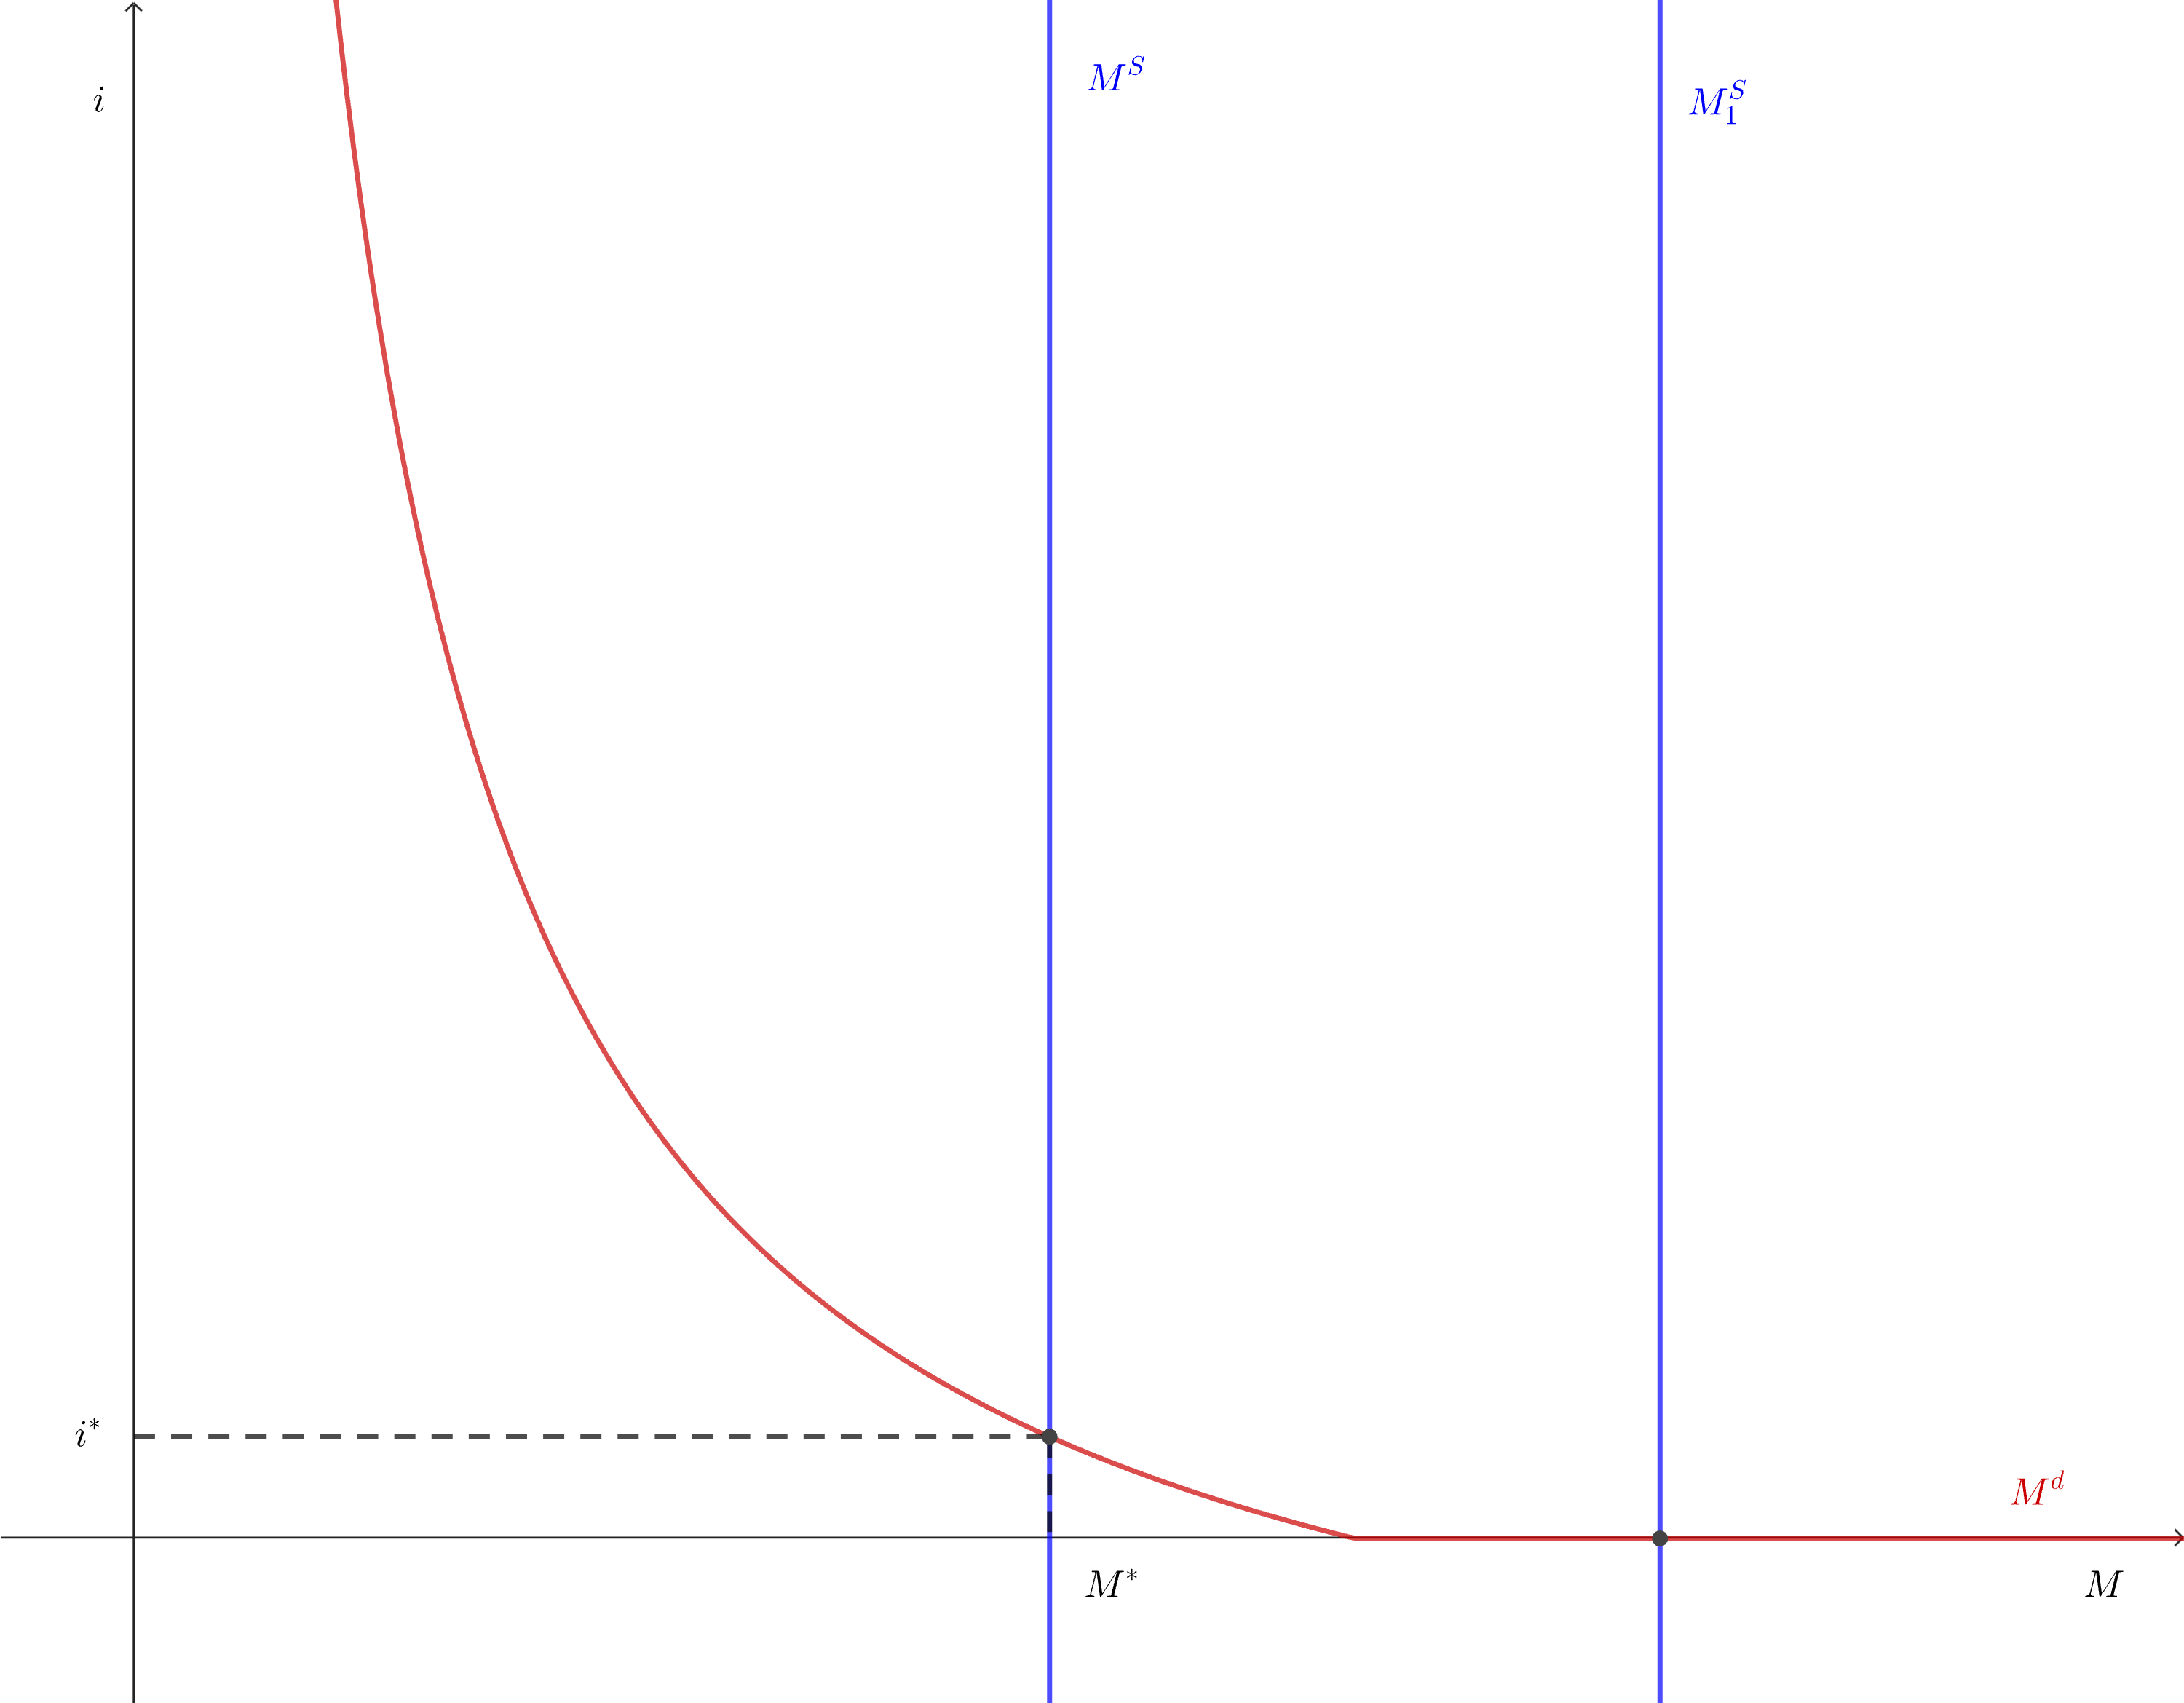
\includegraphics[width=0.5\textwidth]{zlb.png}
    \caption{Zero Lower Bound}
    \label{fig:zlb}
\end{figure}

\begin{example}
	Consider the following money demand function where $Y$ is the nominal income:
	\begin{align*}
		M^d = Y (0.91-5i).
	\end{align*}
	
	\begin{enumerate}[label=(\alph*)]
		\item Suppose that $Y=100$. If the central bank would like to target an interest rate of $2.2\%$, then what should be the money supply?
		\vspace{36pt}
		\item If the nominal income increases to $Y=120$, then how should the central bank change its money supply to maintain the target interest rate?
		\vspace{36pt}
		\item Keep $Y=100$. What is the smallest value of the money supply at which the interest rate is zero?
		\vspace{36pt}
		\item Once the interest rate is zero, can the central bank continue increasing the money supply?
	\end{enumerate}
\end{example}

\end{document}